\chapter{Live Testing}
\label{chapter:testing}

\section{Introduction}
\label{section:introduction}
Towards the end of the implementation of the environment, the project was deployed on a test website and then tested in various schools and grades to ensure full functionality. In this way, feedback for minor adaptions and improvements was gathered, the testing gave an impression of the intermediate result. The testing was designed and arranged that students from a wide range in terms of origin, background, and academic performance were associated with the learning environment, such that authentic and representative feedback could be guaranteed. In the following, the test procedure will be thoroughly examined and explained before the results of the live testing feedback will be presented.

\section{Test Extent}
\label{section:procedure}

\subsection{Test Locations and Grades}
The testing phase was carried out in various schools in different regions of Switzerland. In Zurich, a majority of teachers of the elementary school Entlisberg agreed to participate in the test project. In total, in this school two fourth grades, a third grade and an extra class of specially talented pupil from second to eight grade completed the testing procedure (see figure \ref{fig:testing}). Besides, several groups of specially talented students of both third and fourth grade in the private school Cantaleum Zürich completed the test. A few teachers of other classes from various places also agreed to conduct the live testing by themselves and then provided feedback. In total, over a hundred people tested the platform. The feedback was collected, examined and evaluated in order to improve the learning environment. 

\begin{figure}[H]
    \centering
    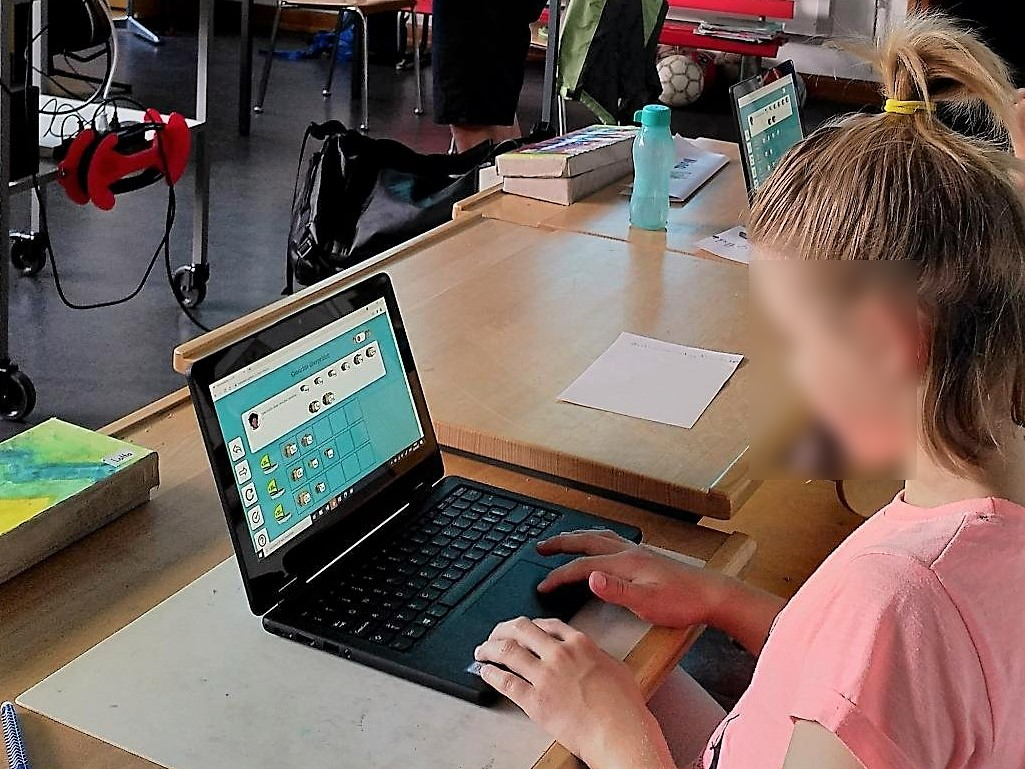
\includegraphics[width=1 \columnwidth]{figures/testing.png}
    \caption{Live testing in a third grade} 
    \label{fig:testing} 
\end{figure}

\subsection{Test Procedure}
The test was organized the following way: In the beginning, the project was presented and its vision and purpose was explained. Then, each student was provided a laptop or tablet and was instructed to solve problem instances for five to ten minutes for each different task type. Each student was advised to try to understand the exercise on their own and check the tutorial in case of problems. At the end, a quick feedback round was conducted, and each student had to fill out an online feedback form. Also, the link to the test website was distributed such that the students would be able to continue solving tasks at home and providing feedback if necessary.

\section{Test Results}
\label{section:results}

\subsection{Impressions and General Feedback}
The general impression of the live testing the teachers and test conductors had was surprisingly positive. The students were eager to solve the tasks and encouraged another to keep going. Some students were quick to understand the exercises and finished soon. Others needed some time to understand the concepts and rules and were not able so solve all the tasks. As for the randomly generated problem instances, some students continuously solved new challenges, while others got stuck with a single problem and needed help or additional explanations. As mentioned before, the range of tested students was very wide in terms of academic performance, such that a small fraction of students seemed unchallenged after a while when other students were overwhelmed with the amount and difficulty of the different task sets. These differences were to be expected, as in the case of the variety within the population. The impression of the testing is confirmed and backed up by some statistical data that will be presented in the next section.

\subsection{Data and Statistics}

The statistical feedback turned out to be thoroughly positive. The feedback form was designed the following way: First, the students had to provide some general information like the grade they attended at that time. The feedback form contained five major paragraphs, where the students had to describe their perception of the learning environment. The paragraphs included questions on how interesting the tasks were, how much fun it was to solve them, if the tasks were easy to understand, if the tutorial was being used and if the amount of exercises was satisfying. Some statistics are shown below to illustrate the feedback. For simplicity's and brevity's sake, only overall results are presented.

In the beginning, the platform had to be evaluated in terms of understandability and intuitiveness. The students were asked how long it took them to understand the exercises, and if they spent much time figuring out what the exact task description was. The result of the survey is visualized in figure \ref{fig:f1}.
Nearly all students considered the tasks to be intuitive and easy to understand. Only a few students did not understand the tasks and had to ask someone for help. These results line up with the impression of the test staff that had to guide single students to understand the requirements of the exercise.


\begin{figure}[H]
    \centering
    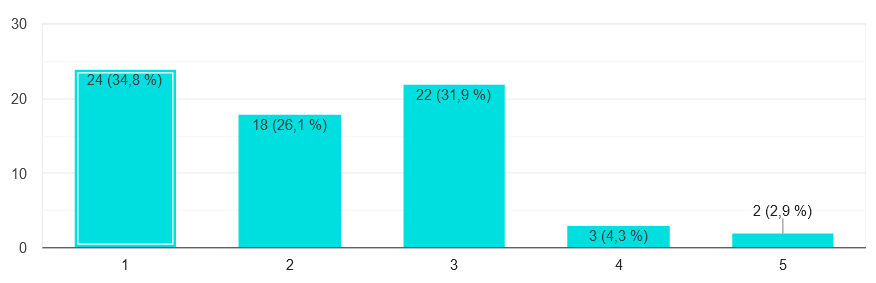
\includegraphics[width=1 \columnwidth]{figures/f1.png}
    \caption{Diagram - On a scale from 1 to 5, how hard were the exercises to understand? 1 corresponds to 'not very hard' and 5 to 'very hard'.} 
    \label{fig:f1} 
\end{figure}

Subsequently, the poll contained a question whether the students opened the tutorial often. This should  help on the one hand to ensure the correctness of the previous survey and on the other hand to know how the students approach a new, unknown task. Recall that the tutorial contains a text and tutorial video that can be opened if the task is unclear. The result of this poll is visualized in figure \ref{fig:f2} and confirmed the previous result that the tasks are well understandable. Additionally, it is evident that the students immediately try to solve the task by testing and trying out by themselves instead of reading the instructions. More than half of the students did not even look once at the tutorial, only few opened it regularly. This also lines up with the perception of the testing staff that noticed that some students did not even read the introductory sentence at the top of the exercise and instead immediately started clicking on the screen until they began to understand how to solve the problem instance.


\begin{figure}[H]
    \centering
    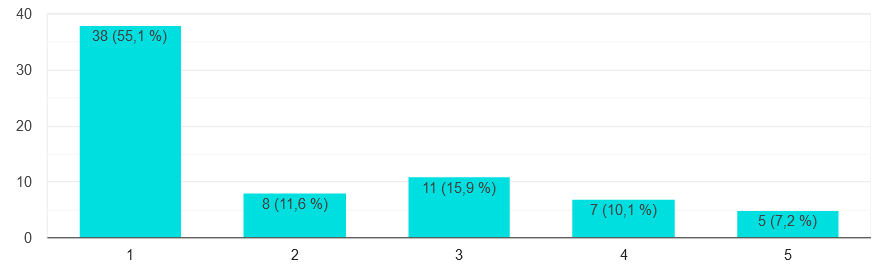
\includegraphics[width=1 \columnwidth]{figures/f2.png}
    \caption{Diagram - On a scale from 1 to 5, how often did you look at the tutorial? 1 corresponds to 'not very often' and 5 to 'very often'.} 
    \label{fig:f2} 
\end{figure}


Next, the satisfaction of the students was to be measured. The user was asked if he or she was content with the way the exercises are designed and if he or she liked the exercises. The result of this poll is visualized in figure \ref{fig:f3} and matched the general feedback of the students that they were very pleased with the learning platform. This was a highly recurring personal feedback among a majority of students. Over 80 percent of the students liked the tasks well to very well. Only a few did not like all of the exercises. An often mentioned reason for this answer was that the exercises were either too simple or too difficult to solve. This result was to be expected, as there are always a few students that are highly intelligent or have problems with reading and understanding assignments.

\begin{figure}[H]
    \centering
    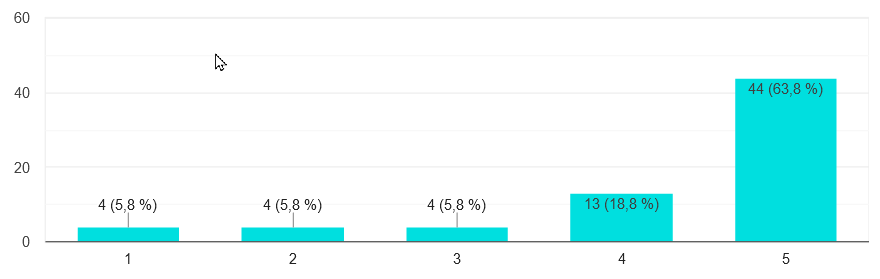
\includegraphics[width=1 \columnwidth]{figures/f3.png}
    \caption{Diagram - On a scale from 1 to 5, how much fun were the exercises? 1 corresponds to 'not so much fun' and 5 to 'much fun'.} 
    \label{fig:f3} 
\end{figure}

Another part of the questionnaire was a section on the attractiveness of the learning environment. The interviewed person had to evaluate how interesting and exciting the tasks were. The result of this poll can be found in figure \ref{fig:f4}. This result was relatively positive, since nearly 90 percent of the students thought the tasks were at least more or less interesting and overall nearly 40 percent rated the exercises to be highly fascinating.

\begin{figure}[H]
    \centering
    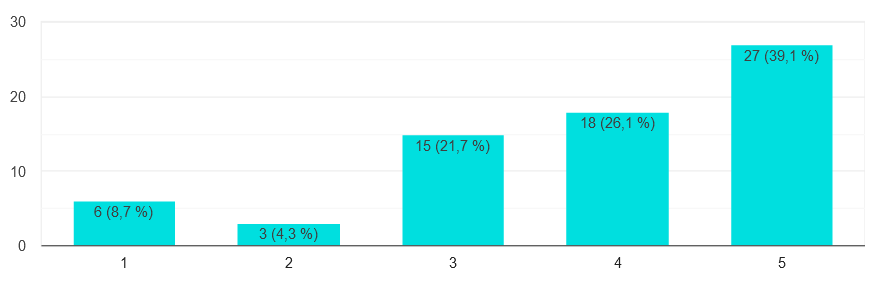
\includegraphics[width=1 \columnwidth]{figures/f4.png}
    \caption{Diagram - On a scale from 1 to 5, how interesting were the exercises? 1 corresponds to 'not very interesting' and 5 to 'very interesting'.}
    \label{fig:f4} 
\end{figure}

Besides this, a section was dedicated to measure the difficulty of the tasks. The user was asked how difficult the exercises were to solve and if the problems were challenging. Figure \ref{fig:f5} gives a detailed overview of the feedback data of this section. The results are as expected normally distributed, that is, there are students that could handle the tasks well while others were challenged by the different task sets. The perception of the task difficulty is normally distributed, with a small tendency towards easiness of the tasks.

\begin{figure}[H]
    \centering
    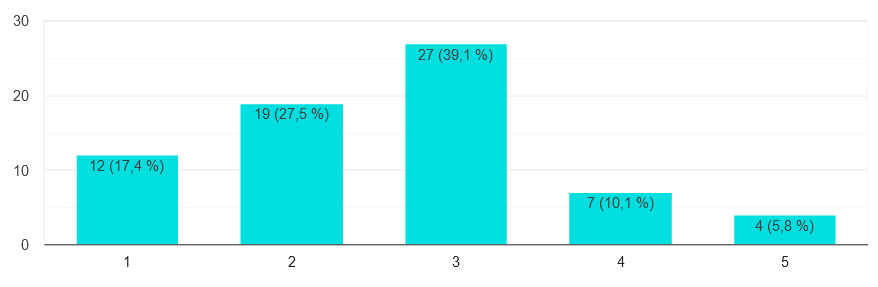
\includegraphics[width=1 \columnwidth]{figures/f5.png}
    \caption{Diagram - On a scale from 1 to 5, how hard were the exercises to solve? 1 corresponds to 'easy' and 5 to 'hard'.}
    \label{fig:f5} 
\end{figure}

In the final evaluation section, the students were asked if the amount of exercises was sufficient. The result of this poll is visualized in figure \ref{fig:f6}. About 3 out of 4 students were content with the variety of tasks.

\begin{figure}[H]
    \centering
    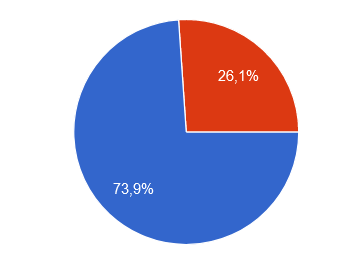
\includegraphics[width=0.5 \columnwidth]{figures/f6.png}
    \caption{Diagram - Are there enough different exercises in the learning environment?} 
    \label{fig:f6} 
\end{figure}
 
In every student feedback, there was then an additional section for written feedback on what one did or did not like and other comments. The results of this part do not deviate from the first five sections: Over 20 percent of the students remarked that they liked everything about the platform, while another 17 percent explicitly mentioned the task set on towers and 15 percent the kiosks task set. The exercises involving weights were mentioned by about 10 percent. Some students appreciated the fact that there are several difficulty levels. Furthermore, about 30 percent of the students explicitly wrote that there is nothing they did not like, while only a few feedbacks mentioned single details that could be improved.

This concludes the testing feedback. In the following, the next steps after the feedback evaluation will be laid out.

\section{Test Conclusion and Consequences}
\label{section:conclusion}

The test results confirmed the supervisor and expert feedback that the exercises are user-friendly and intuitive for elementary school students.

As a consequence of individual and statistical feedback, minor adaptions and corrections were made to the program code in order to enhance the user experience and functionality of the environment. The project could be completely revised and improved according to the feedback. In several task types, the tutorial was revised and extended such that the students can understand the exercise quicker. The introduction as well as the detailed explanation of the task were designed in a way that should even be more intuitive and easier to understand. 
Also, diverse game-play modifications were made to prevent the user from committing false steps in solving the problems. One student even discovered a small bug in the Tower game that allowed the user to place several towers on the same field, which could be immediately fixed. Other students explained what they did not find to be clear enough or what they did not understand at all. This way, real-life experience could be directly included, and the environment could be further enhanced.